\documentclass[10pt,letterpaper]{article}
\usepackage[top=0.85in,left=2.75in,footskip=0.75in]{geometry}

% amsmath and amssymb packages, useful for mathematical formulas and symbols
\usepackage{amsmath,amssymb}

% Use adjustwidth environment to exceed column width (see example table in text)
\usepackage{changepage}

% cite package, to clean up citations in the main text. Do not remove.
\usepackage{cite}

% Use nameref to cite supporting information files (see Supporting Information section for more info)
\usepackage{nameref,hyperref}

% line numbers
\usepackage[right]{lineno}

% ligatures disabled
\usepackage{microtype}
\DisableLigatures[f]{encoding = *, family = * }

% color can be used to apply background shading to table cells only
\usepackage[table]{xcolor}

% array package and thick rules for tables
\usepackage{array}

% Use listings instead of verbatim
\usepackage{listings}
\lstset{
  basicstyle=\ttfamily,
  escapeinside=!!
}

% enumerate package lets us use letters instead of numbers
\usepackage{enumerate}

% create "+" rule type for thick vertical lines
\newcolumntype{+}{!{\vrule width 2pt}}

% create \thickcline for thick horizontal lines of variable length
\newlength\savedwidth
\newcommand\thickcline[1]{%
  \noalign{\global\savedwidth\arrayrulewidth\global\arrayrulewidth 2pt}%
  \cline{#1}%
  \noalign{\vskip\arrayrulewidth}%
  \noalign{\global\arrayrulewidth\savedwidth}%
}

% \thickhline command for thick horizontal lines that span the table
\newcommand\thickhline{\noalign{\global\savedwidth\arrayrulewidth\global\arrayrulewidth 2pt}%
\hline
\noalign{\global\arrayrulewidth\savedwidth}}

\usepackage{color}

% Remove comment for double spacing
%\usepackage{setspace}
%\doublespacing

% Text layout
\raggedright
\setlength{\parindent}{0.5cm}
\textwidth 5.25in
\textheight 8.75in

% Bold the 'Figure #' in the caption and separate it from the title/caption with a period
% Captions will be left justified
\usepackage[aboveskip=1pt,labelfont=bf,labelsep=period,justification=centering,singlelinecheck=off]{caption}
\renewcommand{\figurename}{Fig}

% Use the PLoS provided BiBTeX style
\bibliographystyle{plos2015}

% Remove brackets from numbering in List of References
\makeatletter
\renewcommand{\@biblabel}[1]{\quad#1.}
\makeatother

% Leave date blank
\date{}

% Header and Footer with logo
\usepackage{lastpage,fancyhdr,graphicx}
\usepackage{epstopdf}
\pagestyle{myheadings}
\pagestyle{fancy}
\fancyhf{}
\setlength{\headheight}{27.023pt}
\rfoot{\thepage/\pageref{LastPage}}
\renewcommand{\footrule}{\hrule height 2pt \vspace{2mm}}
\fancyheadoffset[L]{2.25in}
\fancyfootoffset[L]{2.25in}
\lfoot{\sf PLOS}


\begin{document}
\vspace*{0.2in}

\begin{flushleft}
{\Large
\textbf\newline{Twelve Software Design Tips for Data Scientists}
}
\newline
\\
{Greg Wilson}\textsuperscript{1{\ddag}}
\\
\bigskip
\textbf{1} Third Bit\\
{\ddag} Corresponding author, gvwilson@third-bit.com.
\end{flushleft}

\section*{Introduction}

Most people can lift one kilogram,
but would struggle to lift one hundred,
and could not lift a thousand without planning and support.
Similarly,
most researchers can write a few lines of Python, R, or MATLAB to create a plot,
but would struggle to create a program that was a few hundred lines long,
and wouldn't know where to start building an application with many thousands of lines
spread across dozens of modules or packages.

The core challenge is that
\emph{programming in the large} is qualitatively different from \emph{programming in the small}.
as the number of pieces in a program grows,
the number of possible interactions between those pieces grows much more quickly
because $N$ components can be paired in $N^2$ ways.
Programmers who don't manage this complexity
quickly wind up with software that behaves in unexpected (and usually unfortunate) ways
and that cannot be modified without heroic effort.

Most people don't have to write software at that scale,
thanks in large part to an ever-expanding ecosystem of open source software,
but someone has to.
Since many big programs begin life as small scripts,
knowing how to design in the large helps ensure that what's done in the small
is pointed in the right direction.

This paper describes a dozen rules that can help data scientists design large programs.
These rules are taken from published sources,
the author's personal experience,
and discussions over thirty-five years with the creators of widely-used libraries and applications.

\subsection*{Acknowledgments}

The author is grateful to Rebecca Barter,
Neil Brown,
Matthias Bussonnier,
Daniel Chen,
Ildi Czeller,
Bradford Dykes,
Damien Irving,
Mandip Mistry,
Julia Silge,
and Donny Winston
for feedback on early versions of this paper.

\section*{Rule 1: design after the fact}

When we are doing research,
we often don't know what the code should do tomorrow
until we've seen today's results.
It's therefore often pointless to invest as much in up-front planning for our software
as we would in drawing up blueprints for a building.
But this isn't a license to create a tangled mess:
we can and should make it look as though we knew what we were going to do in advance
so that the next person who has to read our code will be able to understand it \cite{Parnas1986}.

\emph{Refactoring} is the process of reorganizing or rewriting code
without changing its externally-visible behavior.
\cite{Fowler2018} describes common refactorings,
such as ``extract function''
(i.e., move some code out of the function its in
and put it in a new function so that it can be called separately)
and ``combine parameters into object''
(which we we will revisit in Rule~5).
Just as the tidying steps in a data pipeline
either convert messy data to a tidy layout or move the data from one tidy layout to another \cite{Wickham2017},
most refactoring operations move code toward or between well-defined patterns \cite{Kerievsky2004}.

\begin{quotation}
  \noindent
  Many designers explain the design of their software
  by recapitulating its history \cite{Brown2011,Brown2012}.
  This is sometimes called \emph{challenge and response}:
  the only way to understand why something works the way it does
  is to understand the problems that existed at the time it was written
  and the tools that were available then.
  Neither programming languages nor existing graphical notations (Rule~10)
  are particularly good at capturing this,
  and while many tools have been written for tracking and managing requirements,
  none have worked well enough that the average programmer would voluntarily adopt them.
\end{quotation}

\section*{Rule 2: design for people's cognitive capacity}

Just as computers have hard drives and RAM,
human brains have long-term and short-term memory \cite{Hermans2021}.
We only have conscious access to short-term memory,
and it is much smaller than most people realize:
early estimates were that the average person could hold
$7{\pm}2$ items in short-term memory at once \cite{Miller1956},
and more recent estimates put its capacity closer to $4{\pm}1$.

The second rule of software design is therefore
to ensure that the number of ``things'' someone has to remember at any time
in order to understand the code they're looking at
fits in short-term memory.
For example,
if a function takes 37 parameters
then the odds are slim
that someone will remember them all and put them in the right order
without a lot of trial and error.
Breaking the function into pieces,
each of which takes only a handful parameters,
reduce the \emph{cognitive load}.
Similarly,
defining default values for most or all of the parameters
will allow people to ignore the details most of the time.

A complementary approach is to create families of functions
that all take similar inputs and outputs
and then combine them using \emph{pipes}.
The pipe operator is one of Unix's key contributions to computing \cite{Kernighan2019},
and the idea has been adopted by many other programming systems,
including the ``tidyverse'' family of packages in R \cite{Wickham2017}.
Where a mathematician would write $f(g(h(x)))$,
a programmer using pipes would write $h(x) | g | f$
so that the functions' names appear in the order in which they are applied.
This may seem like a small change,
but aligning the reading order with execution order
makes the overall effect easier to understand
because the reader only has to ``carry forward'' one piece of information at a time.

\section*{Rule 3: design in coherent levels}

Another rule for designing functions is that
each function should be short, shallow, and single-purpose,
i.e.,
it should implement a single mental operation
so that it only takes up a single slot in short-term memory.
The easiest way to check if this rule is being followed
is to read the function aloud
and ask whether all the steps are at the same conceptual level.
For example,
if I read this Python function aloud:

\begin{verbatim}
 def main():
     config = buildConfiguration(sys.argv)
     state = initializeState(config)
     while config.currentTime < config.haltTime:
         updateState(config, state)
     report(config, state)
\end{verbatim}

\noindent
the comparison of the current time to the halting time in the \texttt{while} loop
feels like it's at a lower level of detail than the function calls.
I would probably rewrite this function as:

\begin{verbatim}
 def main():
     config = buildConfiguration(sys.argv)
     state = initializeState(config)
     while stillEvolving(config, state):
         updateState(config, state)
     report(config, state)
\end{verbatim}

\noindent
This rewrite saves the reader
from having to jump between two different levels of detail
while they're trying to figure out what this function does.

\section*{Rule 4: design for evolution}

The change shown above also makes future evolution easier.
If we decide that the simulation should run until a specified time
\emph{or} until its state has stabilized,
we can make that change in the \texttt{stillEvolving} function
without modifying anything else.

Hiding details like this is another general rule of software design.
Software changes over time because our problems change,
our environments change,
and because our skills improve.
A good design makes independent evolution of parts easier:
basically,
a fix \emph{here} shouldn't require changes \emph{there}.
More realistically,
a change in one place should only require a small number of changes
in a few predictable places.

Software designers achieve this through \emph{information hiding}
and \emph{loose coupling}:

\begin{itemize}

\item
  \emph{Information hiding} means
  putting the data that part of a program needs to do its job in one place,
  and only accessing it through a small set of functions.
  Doing this makes no difference to the computer---by the time it runs the program,
  it's all just a bunch of instructions---but
  people need to understand the program,
  not execute it.

\item
  Doing this allows \emph{loose coupling},
  i.e.,
  those pieces of software can be combined in many different ways
  because none of them depends on the internals of any of the others.

\end{itemize}

Programmers usually implement these principles
by separating \emph{interface} from \emph{implementation}.
The interface specifies what a piece of software can do;
its implementation is how it achieves that,
and no other piece of software should be tied to its implementation details.
The goal is to enable the construction of software components
that can be mixed and matched in the way that USB interfaces allow pieces of hardware to be combined.
Many of the more advanced features of programming languages exist to support or enforce this,
such as being able to derive classes from one another in object-oriented languages like Python,
or creating generic functions that do the same logical thing in different ways for different types of data in languages like R and Julia.

\emph{Design by contract} is one way to enforce this idea \cite{Meyer1994}.
Any function or method can be characterized by
the \emph{pre-conditions} that must be true of its inputs in order for it to run
and the \emph{post-conditions} that it guarantees will be true of its output.
For example,
a function's pre-conditions might be that its input must be
an array of numbers in sorted order,
and its post-condition might be that
the value it returns is one of those elements.

If design by contract is followed,
then a replacement for this function can weaken the pre-conditions
so that it handles a larger set of inputs
and/or strengthen the post-conditions
so that it produces a narrower set of outputs,
but not vice versa.
The first rule ensures that the new function will be able to handle
everything that the old one could;
the second ensures that anything using the old function's output
will still be able to handle everything the new one produces.
Continuing with the previous example,
a new function's pre-conditions could be that it takes any array of numbers,
not just one that is sorted,
and that it produces the largest element in the array.

\section*{Rule 5: group related information together}

If several things are closely related or frequently occur together,
our brains combine them into a ``chunk''
that only takes up one slot in short-term memory.
We can aid this by combining related values into data structures.
For example,
instead of storing the X, Y, and Z coordinates of points separately like this:

\begin{verbatim}
def enclose(x0, y0, z0, x1, y1, z1, nearness):
    ...
\end{verbatim}

\noindent
we can store each point's coordinates in a structure
and write our code like this:

\begin{verbatim}
def enclose(p0, p1, nearness):
    ...
\end{verbatim}

\noindent
Where we need the individual coordinates,
we can refer to them as \texttt{p0.X}, \texttt{p0.Y}, and so on.
Grouping related information together also aids code evolution (Rule~4):
if, for example, we decide to use radial coordinates instead of Cartesian coordinates,
we can change how points are represented without changing most of the functions that pass them around.

\section*{Rule 6: use common patterns}

Some chunks appear so often that we call them ``patterns'' and give them names.
For example,
parasitism and symbiosis take many forms,
and it's impossible to draw a precise boundary between them,
but they are powerful ideas that help us make sense of the world.

Good programmers use \emph{design patterns} to structure their code,
both to reduce the amount of thinking they have to do
and because these patterns have proven to be useful in the past.
Learning patterns helps make someone a better programmer,
i.e.,
there is causation, not just correlation \cite{Tichy2010}.
Conforming to widely-understood patterns also makes code more comprehensible,
just as dividing this paper into sections and a bibliography
that are consistent with what you've read before
makes it easier to read.

Patterns can be found at all scales of programming,
from ``most valuable'' variables \cite{Byckling2005}
and doubly-nested loops to process the elements of two-dimensional arrays
through the filter-group-summarize pattern that is common in data analysis,
to the communicating microservices of today's online applications.
But design patterns can be a mixed blessing.
First,
our brains try so hard to match inputs to patterns that they will sometimes misclassify things.
For example,
it once took me the better part of an hour to spot the error in this code:

\begin{verbatim}
 for (i=0; i<a.width; i++) {
     for (j=0; i<a.height; j++) {
         a[i][j] = cos(abs(a[i][j]) - lemaitre(b_norm, a[j][i]))
     }
 }
\end{verbatim}

The problem is in the second line,
which mistakenly uses the variable \texttt{i} where it should use the variable \texttt{j}.
I couldn't find the mistake because
the code was so close to what it should have been that my brain ``corrected'' what my eyes were seeing,
and because I assumed that since the third line was the most complicated,
the error had to be there.

\begin{quotation}
  In the same way that you shouldn't write a math problem with a function \texttt{x} of variable \texttt{g},
  you should use the same naming conventions as your peers
  to make your code easier to read.
  It doesn't matter what these are,
  any more than it matters whether you spell ``color'' the correct way or the British way;
  what matters is the predictability that comes from consistency.
\end{quotation}

This example illustrates a corollary to Rule~2:
we should write programs that maximize the ratio of unique code to boilerplate.
In most modern languages,
the five lines shown above can be written as:

\begin{verbatim}
a = cos(abs(a) - lemaitre(b_norm, a.transpose()))
\end{verbatim}

\noindent
This version is probably as efficient as the first,
but it is much easier to read and therefore much less likely to mislead.

\section*{Rule 7: design for delivery}

Developer operations (DevOps) has become a buzzword in the last few years.
Like ``data science'' or ``computational thinking'',
the term is popular because people can use it to mean whatever they want,
but the core idea is a good one:
automate compilation, packaging, distribution, deployment, and monitoring
by writing software that operates on or monitors other software \cite{Kim2016,Forsgren2018}.

Investment in automation pays off many times over,
but only if you design things so that they can be automated.
\cite{Taschuk2017} lays out some rules for doing this,
and a few others include:

\begin{enumerate}

\item
  Use the same tools as everyone else who uses your language,
  e.g., \texttt{pip} or \texttt{conda} for Python or \texttt{devtools} for R.
  (One of the weaknesses of modern JavaScript is the number of incompatible options for this.)

\item
  Organize your source files in the way your build system expects
  so that those tools can do their job.

\item
  Handle errors rather than catching and discarding them \cite{Nakshatri2016}.

\item
  Use a logging library rather than \texttt{print} commands
  to report what your program is doing and any errors it has encountered.
  Logging libraries allow you to enable and disable certain categories of messages selectively.
  This is very useful during development,
  but even more so in production,
  since it lets whoever is using your software turn reporting on
  without having to rebuild anything.

\end{enumerate}

\section*{Rule 8: design for testability}

Research software is notoriously difficult to test \cite{Hook2009,Kanewala2014},
in part because its developers often don't know precisely what output the code is supposed to produce.
(As a frustrated chemist once said to the author,
``If I knew what the right answer was, I'd have published it already.'')
It \emph{is} possible to test the ``other 90\%'' of a typical data science application---the parts that
parse input files,
clean up messy data,
and so on,
but only if those parts are designed with testing in mind.

\emph{Legacy code} is software that we're afraid to try to modify
because it's hard to understand and things will break unexpectedly.
A comprehensive set of tests makes us less afraid \cite{Feathers2004},
but we can only create those tests if we design the software in testable pieces.
We can check how well we've done this by asking:

\begin{itemize}
\item
  How easy is it to create a \emph{fixture}
  (i.e., the input that a test runs on)?
\item
  How easy is it to invoke just the behavior we want?
\item
  How easy is it to check the result?
\item
  How easy is it to figure out what ``right'' is?
\item
  How easy is it to delete the feature?
\end{itemize}

For example,
suppose that our program uses species data stored in a large database.
Since our tests only rely on a handful of facts about half a dozen species,
we can:

\begin{enumerate}
\item
  Write a function called \texttt{getSpeciesInfo(speciesId)}
  that gets information about a species given its unique ID
  and put that function in a module called \texttt{production}.
\item
  Create a second module called \texttt{testing}
  that contains a function with the same name
  that takes the same species ID
  and returns a value from a hard-coded lookup table.
  This table only includes the facts we need about the species we use in testing.
\item
  Use a run-time flag to control which of these two modules the program actually loads
  when it runs.
\end{enumerate}

Once again,
funnelling all requests for species information through one function
doesn't just make testing easier today.
It also ensures that if we want to change how information is looked up in future
we are certain that we'll only have to modify one small piece of code.

\section*{Rule 9: design as if code was data}

The insight on which all modern computing is based is that
code is just another kind of data.
Programs are just text files,
and once a program is loaded into memory it is just another data structure:
instead of interpreting its bytes as characters or pixels,
we interpret them as instructions,
but they're still just bytes.

The fact that source code is stored in text files
allows us to build tools that process it,
providing the software is designed with those tools in mind.
Examples include:

\begin{itemize}
\item
  style-checking tools that check that the layout, variable names, and other properties
  conform to coding standards;
\item
  documentation tools that extract specially-formatted comments
  and create cross-referenced manual pages; and
\item
  indexing and navigation tools that enable us to jump directly to
  the definition of a function or variable.
\end{itemize}

It is the second insight---the fact that
a function in memory is just another kind of data---that has the most impact on design.
Just a few of the ways it shows up are:

\begin{itemize}
\item
  Passing functions as arguments to other functions
  so that common operations only have to be written once.
\item
  Storing functions in data structures
  so that new operations can be added to a program
  without changing any of the pre-existing code.
\item
  Loading modules based on configuration parameters
  (as in the earlier example of getting species information).
\end{itemize}

For example,
if we want to count the number of positive values in an array,
we can write:

\begin{verbatim}
def count_positive(array):
    number = 0
    for value in array:
        if value >= 0:
            number = number + 1
    return number
\end{verbatim}

If we want to count the number that are negative,
we could write a \texttt{count\_negative} function that differed by only one character
(replacing the \texttt{>} with \texttt{<}).
Alternatively,
we could write a generic function like this:

\begin{verbatim}
def count_interesting(array, test):
    number = 0
    for value in array:
        if test(value):
            number = number + 1
    return number
\end{verbatim}

\noindent
then put each test in a function like this:

\begin{verbatim}
def is_positive(value):
    return value >= 0
\end{verbatim}

\noindent
and then write something like:

\begin{verbatim}
count_interesting(pressures, is_positive)
\end{verbatim}

Many features in modern languages,
such as lazy evaluation in R or decorators in Python,
leverage this insight,
and taking advantage of it can make code much smaller
and easier to understand---but only if you remember that
what is powerful in the hands of experts is spooky action-at-a-distance for novices.

\begin{quotation}
  The best balance between abstraction and detail
  depends on how much people already know.
  For a novice,
  too many low-level details obscure the meaning,
  while too much abstraction makes it impossible to figure out what's actually going on
  (Figure~\ref{comprehension}).
  As that person gains experience
  they become better able to synthesize meaning from detail
  and translate generalities into specifics,
  but their optimum balance also shifts.
  Software that is easiest for them to understand may not be optimal for someone else.
\end{quotation}

\begin{figure}
  \centering
  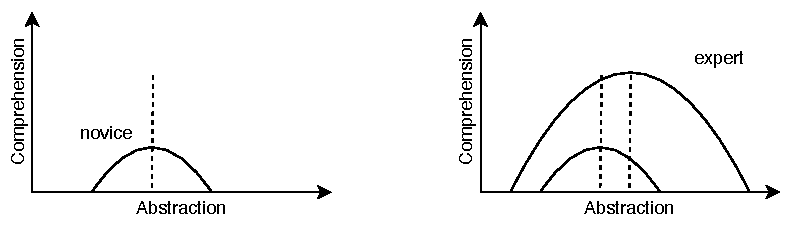
\includegraphics{comprehension.pdf}
  \caption{Comprehension curves for novices and experts}
  \label{comprehension}
\end{figure}

\section*{Rule 10: design graphically}

Many formal graphical notations for software have been designed over the years.
The most famous is the Unified Modeling Language (UML),
but in practice it is taught more often than it is used,
and when it \emph{is} used,
it is usually not in the ways its creators intended \cite{Petre2013}.

However,
many programmers do sketch when they're designing,
and these sketches do help them design.
These sketches are usually not meant as blueprints:
instead,
they help people \emph{externalize cognition},
i.e.,
get their thoughts out where they can see them \cite{Cherubini2007,Petre2016}.
Among the drawings that working programmers often find helpful are:

\begin{itemize}
\item
  flowcharts, which are unfairly maligned \cite{Scanlan1989}
  (Figure~\ref{flowchart});
\item
  entity-relationship diagrams showing how database tables relate to one another
  (Figure~\ref{er-diagram});
\item
  concept maps showing how the designer thinks about the overall problem
  (Figure~\ref{concept-map}); and
\item
  many others,
  such as system architecture diagrams showing the major components of an application
  and use case maps that show how activity flows through an architecture \cite{Reekie2006}.
\end{itemize}

\begin{figure}
  \centering
  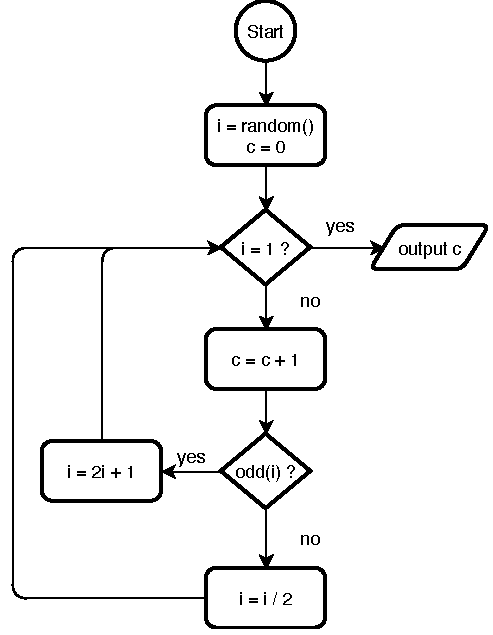
\includegraphics[scale=0.6]{flowchart.pdf}
  \caption{Flowchart}
  \label{flowchart.pdf}
\end{figure}

\begin{figure}
  \centering
  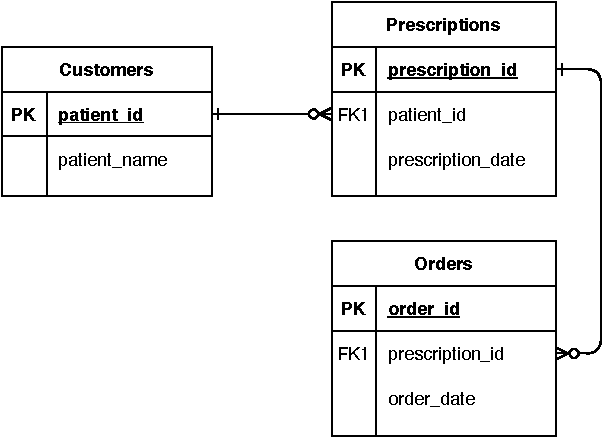
\includegraphics[scale=0.6]{er-diagram.pdf}
  \caption{Entity-relationship diagram}
  \label{er-diagram.pdf}
\end{figure}

\begin{figure}
  \centering
  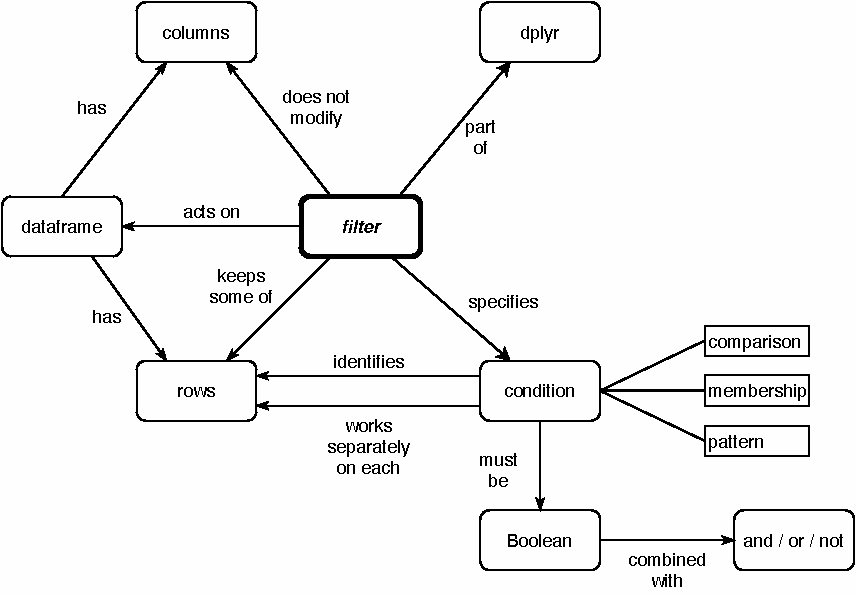
\includegraphics[scale=0.6]{concept-map.pdf}
  \caption{Concept map}
  \label{concept-map.pdf}
\end{figure}

\section*{Rule 11: design with everyone in mind}

If the last few years have taught us anything about software,
it's that fairness, privacy, and security cannot be sprinkled on after the fact.
For example,
if a program is initially designed in a way that allows every user to see everyone else's data,
adding privacy controls later will be expensive and almost certainly buggy.
Programmers to this as the Principle of Least Privilege:
every component in the system should require as few permissions as possible
for as short as possible.

But there is much more to safety-conscious design than just data protection.
For example,
if an application requires users to change their password every few weeks,
\emph{security fatigue} will soon set in
and people will choose less and less secure passwords \cite{Smalls2021}.
Similarly,
programs should not email files to people:
doing that trains them to open attachments,
which is a common channel for attacks.
And every application should allow people to erase data,
which means its data structures and database tables have to be designed to allow for actual erasure,
not just ``mark as inactive''.

Accessibility also can't be sprinkled onto software after the fact.
Close your eyes and try to navigate your institution's website.
Now imagine having to do that all day, every day.
Imagine trying to use a computer when your hands are crippled by arthritis.
Better yet, don't imagine it:
have one of your teammates tape some popsicle sticks to your fingers so you can't bend them
and see what it's like to reply to an email.

Making software accessible doesn't just help people with obvious disabilities:
the population is aging,
and everything you do to help people who are deaf also helps people
who are gradually losing their hearing \cite{Johnson2017}.
A good short guide for accessible design is a set of posters from the UK Home Office \cite{UKHO}.
Each poster in this series lays out a few simple do's and don'ts that will help make your software accessible
to people who are neurodivergent,
use screen readers,
are dyslexic,
have physical or motor challenges, or are hard of hearing.

\section*{Rule 12: design for contribution}

Study after study has shown that diversity improves outcomes in fields from business to healthcare
because many perspectives make for fewer errors \cite{Gompers2018,Gomez2019}.
Good design makes it easier for people who aren't already immersed in your project
to figure out where and how they can contribute to it \cite{Sholler2019},
but just as good programmers consider things like packaging and deployment in their designs,
so too do they think about the factors that influence contribution:

\begin{itemize}

\item
  Software licensing is a design issue,
  since a program can't use libraries whose licenses are incompatible with its own.
  Many designers therefore prefer permissive licenses like the MIT License
  to maximize the number of people who will be able to take advantage of their work.

\item
  Applications that support plug-ins---i.e.,
  that allow people to write small modules that the main program can load and use---are
  often easier for newcomers to contribute to.
  Similarly,
  libraries with strong and consistent conventions for passing data
  (like Unix command-line tools or R's tidyverse functions)
  enable people to start with small contributions.

\end{itemize}

\section*{Conclusion}

\begin{figure}
  \centering
  \includegraphics[width=0.6\textwidth]{derosa.jpg}
  \caption{De Rosa SK Pininfarina (image from \url{https://derosanorthamerica.com/})}
  \label{bicycle}
\end{figure}

Figure~\ref{bicycle} is a De Rosa SK Pininfarina bicycle.
It is not a work of art,
but it can be analyzed and appreciated esthetically.
I believe that programs can be like bicycles:
useful and beautiful at the same time.
We do not yet have as rich a vocabulary for talking about the beauty of software
in the same way that we can talk about the beauty of bicycles or buildings,
but we can still strive to make what we create worthy of appreciation.

\bibliography{12-design}

\end{document}
